

   \subsubsection{Model Instability and Error Surface: Is optimization Always Possible?} 

% direct qoute: Relevance: The function should reflect fundamental properties of the data that the model has to reproduce.
%Speed: The function should be fast to calculate, since
%typically a large amount of error evaluations are performed
%during the search.
%Smoothness: The solution space should be as simple as
%possible, so that the search algorithm can rapidly converge
%to a global optimum. This in general means as little local
%minima as possible.

As previously noted by others \cite{van2007neurofitter}. There are three criteria that govern selection of good fitness error functions these include: speed, smoothness and relevance. In this work, we grappled with some types of error function that were not always smooth. 

%The EFEL signal processing suite was able to produce measurements that fulfilled the speed criteria. 

\subsubsection{Necessary Factors for Reliable Optimization}
Reliable optimization depends on approximately Convex Errors Available to Guide Optimization

Theoretically the largest possible number of constraints would be applied to optimization, because each constraint may provide additional information about the error surface, and may more rapidly exclude great volumes of the solution space. Despite this observation, except in good luck, a successful optimization recipe will not involve the use of all available fitness criterion. This makes the task of model-data fitting far from automatic, in fact human intervention is needed because, not all error signals can be informative guides. 

%\begin{itemize}
    %\item[-] Although there is a large variety of possible errors to use, its rarely a good idea to use all of these errors at once.
    
% NB, this is harder to understand than the residual rheobase error idea.    
    
    One type of error that is can mis-guide, is one who contains a reference point, that is construed relative to each different model parameterization. In an effort to make computer code run without error, under very many different possible conditions, it is tempting to make model measurements that are not objective and unchanging between models. 
    
    A $V_{T}$ threshold my be computed as $(\frac{1}{10})\frac{dV_{M}}{dt}$.
    
    If a neuron model has a spike height below $0mV$, one may be tempted to set a spike detectors threshold as a multiple of $\mu_{V_{M}} - \sigma_{{V_{M}}}$, the mean $V_{M} -$ the standard deviation of the $V_{M}$. This would certainly detect spikes with peaks below $0mV$, and it would work for a wide variety of models too, however, the problem is that because the measurement has a dependency that is relative its self, it is less able to objectively assess waveform differences between  different models.\\
    \\
    For example spike width measurements, need to know the time when the peak of a spike occurred such that it can measure the time between $V_{T}$ and $V_{peak}$. If the method for obtaining spike time, adjusts itself to accommodate model specific differences, in the case when spike time is the same between models, some models will say a spike occurred a bit later, and others a bit earlier, resulting in an unwarranted difference between measurements, which will misguide optimization. The problem can be compounded because other measurements can depend on this measurement, such as spike height, spike width, and $V_{T}$, all of these depend on the spike detection threshold. Which is now not really constant between models.\\
    \\
    %Another cause of misguided errors may involve the recalculating the Rheobase current injection value between different models, there is some error associated with approximating the rheobase current. What is desired is to ascertain the minimal current injection amplitude, which would cause only one spike to fire, but because there is not much time to exhaustively test smaller and smaller values of current amplitude (due to the exploration, exploitation dilemma), one will always settle for an over estimate, one that is somewhere between enough current to cause one or two spikes. The size of this error will vary between models. In addition to this finite precision error, a measurement that is relative to each model, and not objective between models, is a bad idea for the same reason as the model specific measurement for $V_{T}$.\\
    \\
    Spike amplitude will be bigger for some models at their rheobase calculation than other models, especially between models of different input Resistance. Input Resistance will succeed in attenuating greater amplitudes of applied current, however, if a the current succeeds at provoking a spike, the voltage deflection will have a larger peak because of Ohms law: $V=IR$. In this case $V_{M}$, specifically the peak of $V_{M}$ deflection is proportionate to current injection amplitude. So models with different amounts of input resistance will also differ in the peak of the rheobase current injection. However because rheobase is re-calculated per model and because there is finite precision in the rheobase error calculating software it is possible that there will be small regions of error surface, that less accurately encode this relationship.\\
    \\ 
    The situation then compounds when other measurements are taken which depend on rheobase values. An alternative exists where, you sample an error surface using a fixed amount of current preferably at the observed Rheobase current of an experimental cell you are investigating. This would make "Rheobase" a hard constraint, models either spike at the prescribed current, or they don't. Meaning many models are instantly eliminated only because they failed to match Rheobase value, and models that pass this Rheobase test, may score poorly across every other NeuronUnit criteria.
    
    The appeal of applying rheobase as a soft constraint, is that it should widen the scope of finding better models, since models are allowed to perform badly on the rheobase score and good at all other criteria, diverse solutions can compete according to their strengths.%, however, there may be other ways of achieving this.
    
    When applying a fixed rheobase current across many different models only neurons that fail to spike need to be excluded, neurons that fire multiple spikes can still have their spike shapes measured. Additionally, it would be acceptable to run different optimization batches, at different current injection amplitudes, and to federate scores between batches of different current amplitude. The reason why batches need to remain seperate, is that, its only important that error surfaces are convex within the one optimization process. Its okay if two different processes are using different surfaces, as each is blind to the others internal error surface.\\ 
    \\
    %The down side to this approach, is that by distributing the optimization job into batches, it begins to take on an exhaustive nature, and it is not really known, how many current levels would need to be independently explored to achieve good results.\\
    \\
    A different approach was also utilized, where three static quantities of current amplitude $(300pA, 450pA, and 900pA)$ was applied uniformly to all sampled model parameterizations. 
    Another approach, was explored were larger volumes of the solution space were immediately excluded, by way of fixed current.
    %more exclusively
    be to apply a large enough current to invoke spiking in most neurons, and to measure the wave form shape of just one or two spikes in a the resulting spike train.
    
    \subsubsection{Error signals derived from threshold calculations}
    %\begin{itemize}
    %\item[-] 
    A suite of NeuronUnit tests contained two threshold dependent measurements. These were spike half-width, spike height. The treshold was also used to comprize a NU test, so in total three $V_{T}$ measurements were used.
    
    %\item[-] 
    (Ephysiology Feature Extraction Library \cite{EFEL}) EFEL, Allen SDK, and Druckman all contain independently written algorithms for ascertaining modelled neuron $V_{T}$ thresholds calculation code. In all three feature extraction pipelines $V_{T}$ is computed by taking derivative of $V_{M}$
    %\end{itemize}
    
   Another related pitfall is the relationship between the number of free dimensions in the optimization problem versus the number of reliable errors used to constrain the optimization process.
   
   Genetic algorithms are known as derivative free optimizers, since genes are not instructed to take the steepest paths down error slopes, and once inside a local error well a gene is not "stuck" in the well. Although genetic algorithms are robust against being trapped in local minima, however, just like in gradient descent, genetic algorithms can only be guided by information in the error surface. Although genetic algorithms are resilient against local minima, they are nonetheless temporarily misguided by unfortunately positioned local error wells. For this reason Rastrigrins function is used to benchmark the performance of genetic algorithms.\\
   \\
   Rastrigins function has convexity in two scales. On the larger scale the surface has a convex property, on the small scale the function is uniformly pocked with minima wells. Inorder for the GA to optimize Rastrigins function it must be able to exploit the global information of the error surface, and simultaneously the genes will often converge for generations in the minima, but they won't get stuck there because mutation and cross-over will drive the GA to test other less optimal solutions.\\
   \\
   %\begin{figure}
  %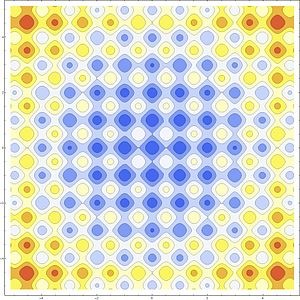
\includegraphics[]{figures/rastagrind.jpg}
  %\caption{}
   %\end{figure}
   
   It is worth noting that although Rastrigrins function is challenging it does not the present the worst gradient to learn from. Worse than Rastrigrins function, are functions that on a large scale are flat, but on the smaller scale contain a high density ripples.
   but lacks this global convex trend, excepting for an abrupt and localised descent to the optima.\\ 
   \\
   Without some first prior knowledge of the error surface, a likely outcome is to attempt optimize on uninformative surfaces. If an uninformative surface is applied, it does not mean that the genetic algorithm will not succeed, it only means that the performance of the GA may be only marginally better than random sampling, or exhaustive search of the error surface.\\
   \\
   Random sampling, sounds bad, however, if the best random solution is digitally stored, and the number of samples applied is less than the possible number of samples in an exhaustive search, random sampling may better resolve the exploitation/exploration dilemna than both gradient descent, and exhaustive search.
{ \hspace*{\fill} \\}      

In the figures below, I describe the spectrum of error surface quality.
\begin{figure}
\centering
\begin{minipage}{.5\textwidth}
  \centering
     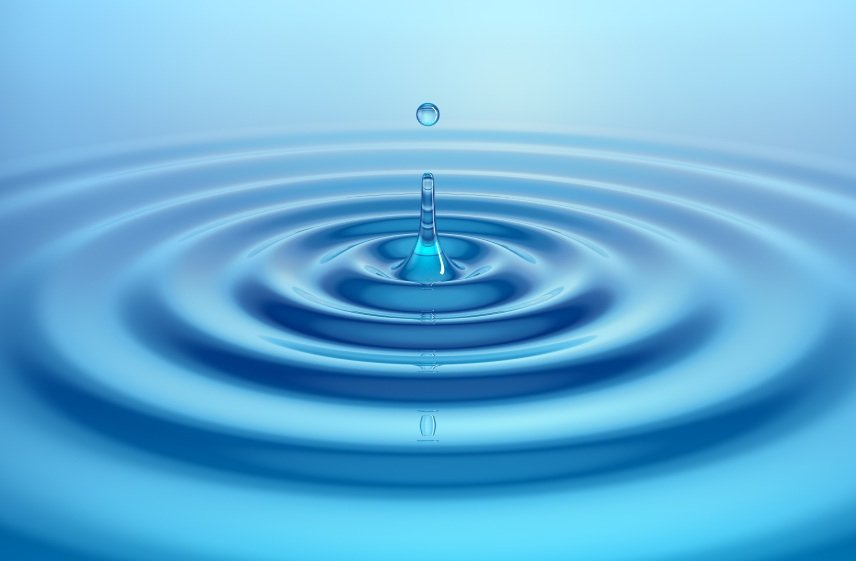
\includegraphics[scale=0.65]{figures/pond_ripple_surface.png}
     \captionof{figure}{In the case of pond ripples the cost function is defined so that the maxima is the optimal location on the surface. Ripples on a body of water are more challenging to optimize, as the water surfaces are approximately flat on the large scale, yet on the small scale maximas will be temporary preoccupy the GAs learning, but outside of those peaks, there is little large scale information to utilize. }
      
      \label{fig:test1}
    \end{minipage}%
    \begin{minipage}{.5\textwidth}
      \centering
      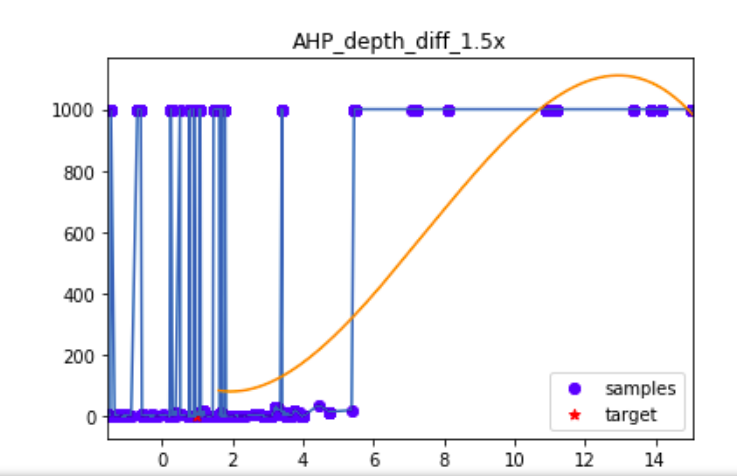
\includegraphics[scale=0.85]{figures/parameter_b_hopeless_surface2.png}
      \captionof{figure}{Similarily parameter b was slowly varied in the Izhikevich model while all other parameters where held constant, the AP1 begin voltage (threshold), was computed for each different model parameterisation of \emph{a}, this resultd in a highly rippled error surface, densely populated by local minima, and with only a very shallow global convex shape}
      \label{fig:test2}
    \end{minipage}
\end{figure}


% Note Help wanted making a professional version, of this known to be unattractive draft/concept figure.
\begin{figure}
\centering

      \label{fig:test1}
    \begin{minipage}{.5\textwidth}
      \centering
      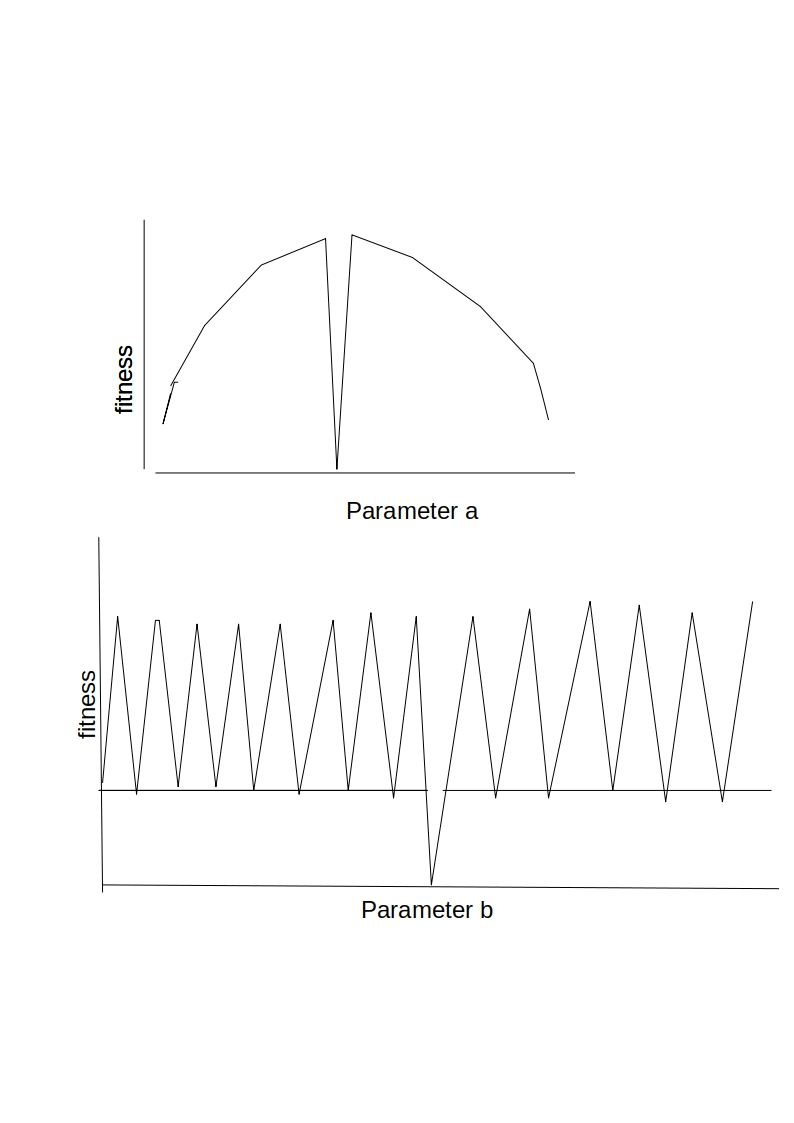
\includegraphics[scale=0.85]{figures/worst_error_surfaces.jpg}
      \captionof{figure}{Rastrigrins function describes a challenging error surface, but one with learnable global features that a genetic algorithm can exploit. It's important to note that there are much worse error surfaces, and these may show up in practice. The first type has actively misleading local and global information. In this context learning is a disadvantage, if the optimizer "learns", then it actually slows obtaining an optimal solution. The second type of error surface (actually a 1D (and upside down) cross section of the 2D pond picture, only actively misleads locally, globally it simply contains no helpful global information. Learning will not be of any assistance in obtaining the optima, but also learning won't actively be a disadvantage either, the Genetic Algorithm, will simply behave as a random sampling/testing algorithm, the GA will find the optimum in time, but possibly not as quickly or reliably as exhaustive search would. The second figure is a cross section of the pond ripple argument}
      \label{fig:test2}
    \end{minipage}
\end{figure}

\begin{figure}
\centering


    
    \begin{minipage}{.5\textwidth}
      \centering
      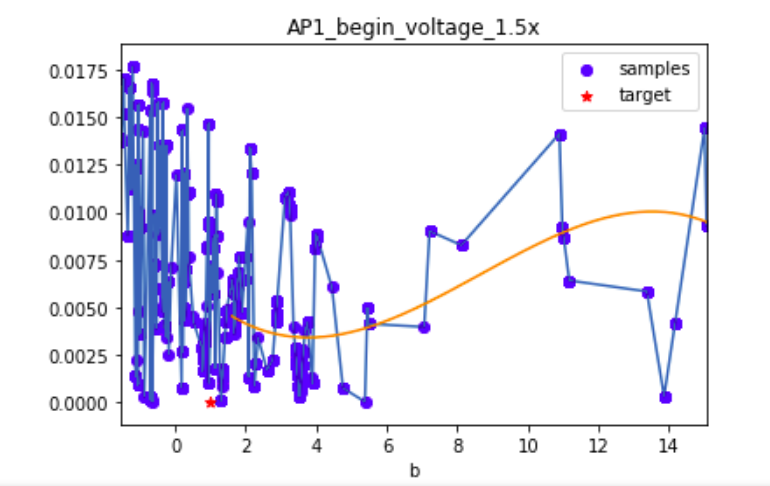
\includegraphics[scale=0.85]{figures/parameter_b_hopeless_surface.png}
      \captionof{figure}{Similarily parameter b was slowly varied in the Izhikevich model while all other parameters where held constant, the AP1 begin voltage (threshold), was computed for each different model parameterisation of \emph{a}, this resultd in a highly rippled error surface, densely populated by local minima, and with only a very shallow global convex shape}
      \label{fig:test2}
    \end{minipage}

    \begin{minipage}{.5\textwidth}
      \centering
      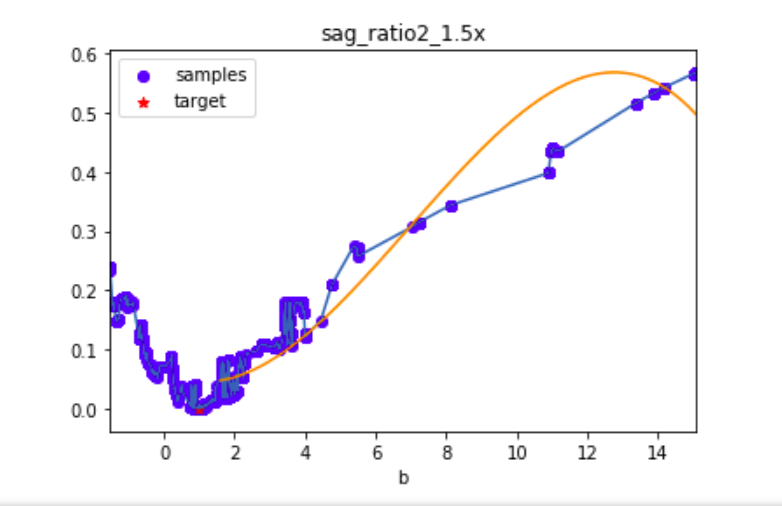
\includegraphics[scale=0.85]{figures/parameter_b_friendly_surface.png}
      \captionof{figure}{This is an example of a useable and tractable error surface, it has learnable global and local information, as long as not all error surfaces in the multiobjective collection of constraints, this surface is likely to be a valueable addition to the optimizer suite}
      \label{fig:test2}
    \end{minipage}


\end{figure}



     
   When considering 2D relationships between single parameters and single objective functions, ideally each objective function might contribute helpful information, that on mass boosts the total amount of helpful information. For-instance some 2D error mappings, may contain one or more local minima, but in the same region a different error mapping could lack the well, meaning that at least one out of two error functions contribute incentive to stride across a minima. The mapping that contains wells, might still be useful to guide optimization, as it may also lack minima in regions were the counterpart has them, additionally the counterpart mapping may have regions of $~0.0$ gradient where the other mapping contains significant gradient.
   
   % I am not sure if its impossible to make progress.
   Through shear luck it is possible to optimize well without prior knowledge of error surfaces, although such a strategy is not recommended. If prior knowledge of an error surface is prohibited, evolutionary algorithms are definitely a more likely to work than gradient descent.
   
   In a multi objective paradigm, an optimizer could achieve satisfactory solutions when $\frac{3}{4}$ objectives are cogent. If the $4$th objective is un-informative, but not actively misleading, it may just slow down the speed of convergence.
   
   If the $4$ objective is actively misleading, then a genetic algorithm will likely find a satisfactory solution, by compromising with the dominant $3$ objective functions, and also sampling believed to be "bad" surfaces because of mutation and cross over. Speed of convergence should also be expected to be slower than otherwise. With $\frac{2}{4}$ actively misleading error surfaces, optimization is not expected to work, and it may be slower than psuedo random sampling.
   
   It is almost impossible to make progress without some prior knowledge of the error surfaces, as knowledge of the error surface is a prerequisite for constraining optimization. Not all surfaces, provide equally useful information. There are spectrums of surface quality between convex traingular or parabolic depressions acting as the best solution surfaces, and flat functions. 
   

\subsubsection{Parameter Boundaries}
When setting parameter boundaries there is a dilemma: If the upper and lower parameter margins are closer together than necessary, then optimized models may be deprived of the scope they need to reach their best fit. 

\begin{figure}
    \centering
    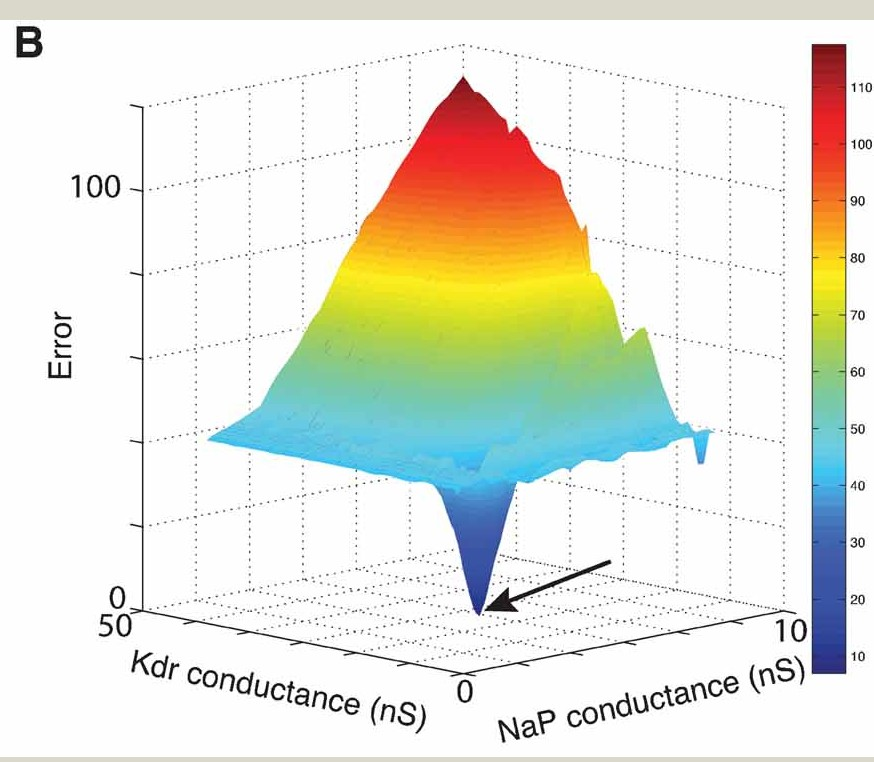
\includegraphics{figures/fninf-01-001-g009.jpg}
    \caption{Caption}
    \label{fig:best_at_edge}
\end{figure}

Consider figure B in the inset \ref{fig:best_at_edge}, in figure B a global minima is positioned at the intersection two parameter edges in both $Kdr$ and $NaP$. It would be easy to formulate the same optimization problem to have truncated scope about the extremes of $NaP$ and $Kdr$ and as a consequence to miss the uniquely positioned global optima situated on the intersection. The alternative optima that would be reported is the broad spanning region that shares the same second lowest value to the optima. The genetic algorithm

On the other hand if the boundaries are too far apart, then the governing equations of the model may yield unstable solutions, which may impair the tractibility of the error surface as I will describe below.

Error surface tractability can be compromized in two ways.
Type \textbf{1} solutions to governing equations may contain "not a number" (NaN) or infinity value. The optimizer conventionally interprets more positive numbers as worse. Inside the optimization framework infinity or NaN values are converted to a nominal value of $100.0$, the worst conceivable model score. If more than one gene scores at $100$, then there will be regions of flat error surface. %Although genetic algorithms are not pre-determined to take the steepest path down an error slope, 
%All optimization algorithms are sensitive to the informativeness of error surface, therefore a flat error surface is unhelpful in both gradient descent and genetic algorithms, 
When error surface is flat it is uninformative. 
Because, model-solution instability can occur when the optimizer uses model parameters are used outside of the models intended scope, it is tempting to think of these flat regions as a flat ledge that neatly encases the error hyper volume like in the figure below \ref{fig:cliff}, unfortunately however, because each model has a large number of parameters typically $>10$, any particular model instance, only one of these parameters need be evaluating an unstable model when exceeding a margin, the rest of the parameters may be in the middle of their range, and so such a ledge may actually be experienced as a hyper dimensional "tower", this tower could actually be experienced in the middle of parameter space in 10 out of 11 parameters, while still being on at the edge for only the 11th parameter.


\begin{figure}
    \centering
    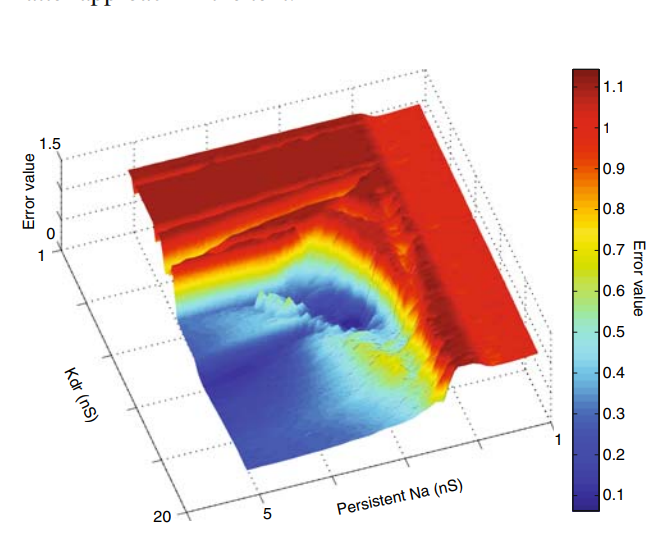
\includegraphics{figures/cliff}
    \caption{Cliff ledge in 2D error surface}
    \label{fig:cliff}
\end{figure}


Although we are considering single points, and not surfaces, very often if a point is unstable, its neighbours are also unstable, in this way points of instability tend to be a constituents of larger regions of surface that add up to towers, cliffs and ledges such as those in seen here {fig:cliff}.

One or more cliffs or towers situated in the middle of the error surface, poses problems for efficient optimization, where genes learn the general shape of an error surface. Such cliffs and ledges will mislead the optimizer and they will act exactly like the ripples discussed briefly before in this work.

Type \textbf{2}: While some towers can be circumvented by choosing slimmer parameter margins, other ledges and ripples of these ledges are implied by the types of model and test combinations. Rather than being avoidable, they are a feature of the complex problem that the optimizer is tasked with solving.

Forinstance, in bursting regimes of the Izhikevich model, where models deliberately produce close to unstable limit cycles. When surpassing the threshold to cause spiking, the slightest increment of current  will illicit not a single spike but a burst of ten.

Rheobase values will be undetermined, because the a the smallest current injection value to cause only one spike does not exist. The models rheobase value will be assigned to 100, and a tower will punctuate, the error surface possibly in the middle of the Izhikevich parameter hypervolume. The experience of sampling this tower, will visible in post evaluation of the genetic algorithms learning performance. It will appear as a one or several unexpected peaks late in the genetic algorithms learning.

This means that even under the most tractible conditions when evaluating the performance of genetic algorithm learning, the rapidity of genetic convergence will vary depending on which constraints are chosen, and the regime that the neuronal model is currently sampling from (the models parameters). There will be regions of genetic learning when models will encode high local pockets of error, or "towers" in the middle of the hyper-volume, and if these towers are significantly wide or densely populated, the genetic algorithms learning will be visibly diminished to a random sampling algorithm. What is more, these discontinuties under some circumstances may act to lesion error surfaces and inhibit migration of models from side to side. Movement over cliffs of course will still ultimately occur due to stochastic pressure in gene mutation.

A possible solution to the dilemma of narrow parameter boundaries is to write an algorithm that slowly samples models by expanding beyond known to stable boundaries, and reports back on model stability. In this manner one can programmatically determine maximum parameter boundaries, however, model equations used here, do exhibit some higher order sensativity by changing a second intermediate parameter. Very quickly this approach to finding the maximum scope of a parameter may begin to look like exhaustive search.

Another programmatic approach is to use a wide variety of models and tests, and to accept that for some model-test combinations, for some regions of parameter space, genetic algorithms are at worst  randomly stumbling upon satisfactory solutions.
